% Options for packages loaded elsewhere
\PassOptionsToPackage{unicode}{hyperref}
\PassOptionsToPackage{hyphens}{url}
\PassOptionsToPackage{dvipsnames,svgnames*,x11names*}{xcolor}
%
\documentclass[
]{article}
\usepackage{lmodern}
\usepackage{amssymb,amsmath}
\usepackage{ifxetex,ifluatex}
\ifnum 0\ifxetex 1\fi\ifluatex 1\fi=0 % if pdftex
  \usepackage[T1]{fontenc}
  \usepackage[utf8]{inputenc}
  \usepackage{textcomp} % provide euro and other symbols
\else % if luatex or xetex
  \usepackage{unicode-math}
  \defaultfontfeatures{Scale=MatchLowercase}
  \defaultfontfeatures[\rmfamily]{Ligatures=TeX,Scale=1}
\fi
% Use upquote if available, for straight quotes in verbatim environments
\IfFileExists{upquote.sty}{\usepackage{upquote}}{}
\IfFileExists{microtype.sty}{% use microtype if available
  \usepackage[]{microtype}
  \UseMicrotypeSet[protrusion]{basicmath} % disable protrusion for tt fonts
}{}
\makeatletter
\@ifundefined{KOMAClassName}{% if non-KOMA class
  \IfFileExists{parskip.sty}{%
    \usepackage{parskip}
  }{% else
    \setlength{\parindent}{0pt}
    \setlength{\parskip}{6pt plus 2pt minus 1pt}}
}{% if KOMA class
  \KOMAoptions{parskip=half}}
\makeatother
\usepackage{xcolor}
\IfFileExists{xurl.sty}{\usepackage{xurl}}{} % add URL line breaks if available
\IfFileExists{bookmark.sty}{\usepackage{bookmark}}{\usepackage{hyperref}}
\hypersetup{
  pdftitle={Week 3 - Homework},
  pdfauthor={STAT 420, Summer 2020, D. Unger},
  colorlinks=true,
  linkcolor=Maroon,
  filecolor=Maroon,
  citecolor=Blue,
  urlcolor=cyan,
  pdfcreator={LaTeX via pandoc}}
\urlstyle{same} % disable monospaced font for URLs
\usepackage[margin=1in]{geometry}
\usepackage{color}
\usepackage{fancyvrb}
\newcommand{\VerbBar}{|}
\newcommand{\VERB}{\Verb[commandchars=\\\{\}]}
\DefineVerbatimEnvironment{Highlighting}{Verbatim}{commandchars=\\\{\}}
% Add ',fontsize=\small' for more characters per line
\usepackage{framed}
\definecolor{shadecolor}{RGB}{248,248,248}
\newenvironment{Shaded}{\begin{snugshade}}{\end{snugshade}}
\newcommand{\AlertTok}[1]{\textcolor[rgb]{0.94,0.16,0.16}{#1}}
\newcommand{\AnnotationTok}[1]{\textcolor[rgb]{0.56,0.35,0.01}{\textbf{\textit{#1}}}}
\newcommand{\AttributeTok}[1]{\textcolor[rgb]{0.77,0.63,0.00}{#1}}
\newcommand{\BaseNTok}[1]{\textcolor[rgb]{0.00,0.00,0.81}{#1}}
\newcommand{\BuiltInTok}[1]{#1}
\newcommand{\CharTok}[1]{\textcolor[rgb]{0.31,0.60,0.02}{#1}}
\newcommand{\CommentTok}[1]{\textcolor[rgb]{0.56,0.35,0.01}{\textit{#1}}}
\newcommand{\CommentVarTok}[1]{\textcolor[rgb]{0.56,0.35,0.01}{\textbf{\textit{#1}}}}
\newcommand{\ConstantTok}[1]{\textcolor[rgb]{0.00,0.00,0.00}{#1}}
\newcommand{\ControlFlowTok}[1]{\textcolor[rgb]{0.13,0.29,0.53}{\textbf{#1}}}
\newcommand{\DataTypeTok}[1]{\textcolor[rgb]{0.13,0.29,0.53}{#1}}
\newcommand{\DecValTok}[1]{\textcolor[rgb]{0.00,0.00,0.81}{#1}}
\newcommand{\DocumentationTok}[1]{\textcolor[rgb]{0.56,0.35,0.01}{\textbf{\textit{#1}}}}
\newcommand{\ErrorTok}[1]{\textcolor[rgb]{0.64,0.00,0.00}{\textbf{#1}}}
\newcommand{\ExtensionTok}[1]{#1}
\newcommand{\FloatTok}[1]{\textcolor[rgb]{0.00,0.00,0.81}{#1}}
\newcommand{\FunctionTok}[1]{\textcolor[rgb]{0.00,0.00,0.00}{#1}}
\newcommand{\ImportTok}[1]{#1}
\newcommand{\InformationTok}[1]{\textcolor[rgb]{0.56,0.35,0.01}{\textbf{\textit{#1}}}}
\newcommand{\KeywordTok}[1]{\textcolor[rgb]{0.13,0.29,0.53}{\textbf{#1}}}
\newcommand{\NormalTok}[1]{#1}
\newcommand{\OperatorTok}[1]{\textcolor[rgb]{0.81,0.36,0.00}{\textbf{#1}}}
\newcommand{\OtherTok}[1]{\textcolor[rgb]{0.56,0.35,0.01}{#1}}
\newcommand{\PreprocessorTok}[1]{\textcolor[rgb]{0.56,0.35,0.01}{\textit{#1}}}
\newcommand{\RegionMarkerTok}[1]{#1}
\newcommand{\SpecialCharTok}[1]{\textcolor[rgb]{0.00,0.00,0.00}{#1}}
\newcommand{\SpecialStringTok}[1]{\textcolor[rgb]{0.31,0.60,0.02}{#1}}
\newcommand{\StringTok}[1]{\textcolor[rgb]{0.31,0.60,0.02}{#1}}
\newcommand{\VariableTok}[1]{\textcolor[rgb]{0.00,0.00,0.00}{#1}}
\newcommand{\VerbatimStringTok}[1]{\textcolor[rgb]{0.31,0.60,0.02}{#1}}
\newcommand{\WarningTok}[1]{\textcolor[rgb]{0.56,0.35,0.01}{\textbf{\textit{#1}}}}
\usepackage{longtable,booktabs}
% Correct order of tables after \paragraph or \subparagraph
\usepackage{etoolbox}
\makeatletter
\patchcmd\longtable{\par}{\if@noskipsec\mbox{}\fi\par}{}{}
\makeatother
% Allow footnotes in longtable head/foot
\IfFileExists{footnotehyper.sty}{\usepackage{footnotehyper}}{\usepackage{footnote}}
\makesavenoteenv{longtable}
\usepackage{graphicx,grffile}
\makeatletter
\def\maxwidth{\ifdim\Gin@nat@width>\linewidth\linewidth\else\Gin@nat@width\fi}
\def\maxheight{\ifdim\Gin@nat@height>\textheight\textheight\else\Gin@nat@height\fi}
\makeatother
% Scale images if necessary, so that they will not overflow the page
% margins by default, and it is still possible to overwrite the defaults
% using explicit options in \includegraphics[width, height, ...]{}
\setkeys{Gin}{width=\maxwidth,height=\maxheight,keepaspectratio}
% Set default figure placement to htbp
\makeatletter
\def\fps@figure{htbp}
\makeatother
\setlength{\emergencystretch}{3em} % prevent overfull lines
\providecommand{\tightlist}{%
  \setlength{\itemsep}{0pt}\setlength{\parskip}{0pt}}
\setcounter{secnumdepth}{-\maxdimen} % remove section numbering

\title{Week 3 - Homework}
\author{STAT 420, Summer 2020, D. Unger}
\date{}

\begin{document}
\maketitle

\hypertarget{directions}{%
\section{Directions}\label{directions}}

Students are encouraged to work together on homework. However, sharing,
copying or providing any part of a homework solution or code is an
infraction of the University's rules on Academic Integrity. Any
violation will be punished as severely as possible.

\begin{itemize}
\tightlist
\item
  Be sure to remove this section if you use this \texttt{.Rmd} file as a
  template.
\item
  You may leave the questions in your final document.
\end{itemize}

\begin{center}\rule{0.5\linewidth}{0.5pt}\end{center}

\hypertarget{exercise-1-using-lm-for-inference}{%
\subsection{\texorpdfstring{Exercise 1 (Using \texttt{lm} for
Inference)}{Exercise 1 (Using lm for Inference)}}\label{exercise-1-using-lm-for-inference}}

For this exercise we will use the \texttt{cats} dataset from the
\texttt{MASS} package. You should use \texttt{?cats} to learn about the
background of this dataset.

\textbf{(a)} Fit the following simple linear regression model in
\texttt{R}. Use heart weight as the response and body weight as the
predictor.

\[
Y_i = \beta_0 + \beta_1 x_i + \epsilon_i
\]

Store the results in a variable called \texttt{cat\_model}. Use a \(t\)
test to test the significance of the regression. Report the following:

\begin{itemize}
\tightlist
\item
  The null and alternative hypotheses
\item
  The value of the test statistic
\item
  The p-value of the test
\item
  A statistical decision at \(\alpha = 0.05\)
\item
  A conclusion in the context of the problem
\end{itemize}

When reporting these, you should explicitly state them in your document,
not assume that a reader will find and interpret them from a large block
of \texttt{R} output.

\begin{Shaded}
\begin{Highlighting}[]
\KeywordTok{library}\NormalTok{(MASS)}
\NormalTok{cat_model =}\StringTok{ }\KeywordTok{lm}\NormalTok{(Hwt }\OperatorTok{~}\StringTok{ }\NormalTok{Bwt, }\DataTypeTok{data =}\NormalTok{ cats)}
\KeywordTok{summary}\NormalTok{(cat_model)}\OperatorTok{$}\NormalTok{coefficients}
\end{Highlighting}
\end{Shaded}

\begin{verbatim}
##               Estimate Std. Error    t value     Pr(>|t|)
## (Intercept) -0.3566624  0.6922770 -0.5152019 6.072131e-01
## Bwt          4.0340627  0.2502615 16.1193908 6.969045e-34
\end{verbatim}

\begin{Shaded}
\begin{Highlighting}[]
\KeywordTok{summary}\NormalTok{(cat_model)}\OperatorTok{$}\NormalTok{coefficients[}\StringTok{"Bwt"}\NormalTok{, }\StringTok{"t value"}\NormalTok{]}
\end{Highlighting}
\end{Shaded}

\begin{verbatim}
## [1] 16.11939
\end{verbatim}

\begin{Shaded}
\begin{Highlighting}[]
\KeywordTok{summary}\NormalTok{(cat_model)}\OperatorTok{$}\NormalTok{coefficients[}\StringTok{"Bwt"}\NormalTok{, }\StringTok{"Pr(>|t|)"}\NormalTok{]}
\end{Highlighting}
\end{Shaded}

\begin{verbatim}
## [1] 6.969045e-34
\end{verbatim}

H0: beta\_one = 0

H1: beta\_one != 0

The value of the test statistic is 16.11939

The p-value of the test is 6.969045e-34

Statistical Decision at alpha = 0.05 is Reject H0

Conclusion in the context of the problem: there exists a linear
relationship between heart weight and body weight

\textbf{(b)} Calculate a 95\% confidence interval for \(\beta_1\). Give
an interpretation of the interval in the context of the problem.

\begin{Shaded}
\begin{Highlighting}[]
\KeywordTok{confint}\NormalTok{(cat_model, }\StringTok{"Bwt"}\NormalTok{, }\DataTypeTok{level =} \FloatTok{0.95}\NormalTok{)}
\end{Highlighting}
\end{Shaded}

\begin{verbatim}
##        2.5 %   97.5 %
## Bwt 3.539343 4.528782
\end{verbatim}

Confidence interval for \(\beta_1\) is inbetween (3.539343, 4.528782).

We are 95\% confident that given a 1 KG increase in the body weight, the
avarage heart weight will be between 3.539343 and 4.528782. Since the
interval doesn't have a zero value, it is not possible to have
\(\beta_1\) a zero value.

\textbf{(c)} Calculate a 90\% confidence interval for \(\beta_0\). Give
an interpretation of the interval in the context of the problem.

\begin{Shaded}
\begin{Highlighting}[]
\KeywordTok{confint}\NormalTok{(cat_model, }\StringTok{"(Intercept)"}\NormalTok{, }\DataTypeTok{level =} \FloatTok{0.90}\NormalTok{)}
\end{Highlighting}
\end{Shaded}

\begin{verbatim}
##                   5 %      95 %
## (Intercept) -1.502834 0.7895096
\end{verbatim}

Confidence interval for \(\beta_0\) is inbetween (-1.502834, 0.7895096).

We are 90\% confident that for a body weight of 0 KG, the average heart
weight will be between -1.502834 and 0.7895096. Practically speaking it
wouldn't make much sense.

\textbf{(d)} Use a 90\% confidence interval to estimate the mean heart
weight for body weights of 2.1 and 2.8 kilograms. Which of the two
intervals is wider? Why?

\begin{Shaded}
\begin{Highlighting}[]
\NormalTok{hwt_ci =}\StringTok{ }\KeywordTok{predict}\NormalTok{(cat_model, }\DataTypeTok{newdata =} \KeywordTok{data.frame}\NormalTok{(}\DataTypeTok{Bwt =} \KeywordTok{c}\NormalTok{(}\FloatTok{2.1}\NormalTok{, }\FloatTok{2.8}\NormalTok{)), }\DataTypeTok{interval =} \KeywordTok{c}\NormalTok{(}\StringTok{"confidence"}\NormalTok{), }\DataTypeTok{level =} \FloatTok{0.90}\NormalTok{)}
\NormalTok{hwt_ci}
\end{Highlighting}
\end{Shaded}

\begin{verbatim}
##         fit       lwr       upr
## 1  8.114869  7.787882  8.441856
## 2 10.938713 10.735843 11.141583
\end{verbatim}

We are 90\% confident that the mean heart weight for body weights 2.1
and 2.8 KG is in the intervals of (7.599225, 8.630513) and (10.618796,
11.258630) respectively

\begin{Shaded}
\begin{Highlighting}[]
\KeywordTok{mean}\NormalTok{(cats}\OperatorTok{$}\NormalTok{Bwt)}
\end{Highlighting}
\end{Shaded}

\begin{verbatim}
## [1] 2.723611
\end{verbatim}

\begin{Shaded}
\begin{Highlighting}[]
\KeywordTok{range}\NormalTok{(cats}\OperatorTok{$}\NormalTok{Bwt)}
\end{Highlighting}
\end{Shaded}

\begin{verbatim}
## [1] 2.0 3.9
\end{verbatim}

\begin{Shaded}
\begin{Highlighting}[]
\NormalTok{diff_}\DecValTok{21}\NormalTok{ =}\StringTok{ }\NormalTok{(hwt_ci[}\DecValTok{1}\NormalTok{,}\DecValTok{3}\NormalTok{] }\OperatorTok{-}\StringTok{ }\NormalTok{hwt_ci[}\DecValTok{1}\NormalTok{,}\DecValTok{2}\NormalTok{])}
\NormalTok{diff_}\DecValTok{28}\NormalTok{ =}\StringTok{ }\NormalTok{(hwt_ci[}\DecValTok{2}\NormalTok{,}\DecValTok{3}\NormalTok{] }\OperatorTok{-}\StringTok{ }\NormalTok{hwt_ci[}\DecValTok{2}\NormalTok{,}\DecValTok{2}\NormalTok{])}
\NormalTok{diff_}\DecValTok{21} \OperatorTok{>}\StringTok{ }\NormalTok{diff_}\DecValTok{28}
\end{Highlighting}
\end{Shaded}

\begin{verbatim}
## [1] TRUE
\end{verbatim}

body weight of 2.1 KG interval is larger as it is further from the
sample mean body weight. Also the body weights are within the range of
observed body weights.

\textbf{(e)} Use a 90\% prediction interval to predict the heart weight
for body weights of 2.8 and 4.2 kilograms.

\begin{Shaded}
\begin{Highlighting}[]
\NormalTok{hwt_ci =}\StringTok{ }\KeywordTok{predict}\NormalTok{(cat_model, }\DataTypeTok{newdata =} \KeywordTok{data.frame}\NormalTok{(}\DataTypeTok{Bwt =} \KeywordTok{c}\NormalTok{(}\FloatTok{2.8}\NormalTok{, }\FloatTok{4.2}\NormalTok{)), }\DataTypeTok{interval =} \KeywordTok{c}\NormalTok{(}\StringTok{"prediction"}\NormalTok{), }\DataTypeTok{level =} \FloatTok{0.90}\NormalTok{)}
\NormalTok{hwt_ci}
\end{Highlighting}
\end{Shaded}

\begin{verbatim}
##        fit       lwr      upr
## 1 10.93871  8.525541 13.35189
## 2 16.58640 14.097100 19.07570
\end{verbatim}

We are 90\% confident that the new observation for body weights 2.8 and
4.2 KG is in the intervals of (5.688109, 10.54163) and (8.525541,
13.35189) respectively

\begin{Shaded}
\begin{Highlighting}[]
\NormalTok{diff_}\DecValTok{28}\NormalTok{ =}\StringTok{ }\NormalTok{(hwt_ci[}\DecValTok{1}\NormalTok{,}\DecValTok{3}\NormalTok{] }\OperatorTok{-}\StringTok{ }\NormalTok{hwt_ci[}\DecValTok{1}\NormalTok{,}\DecValTok{2}\NormalTok{])}
\NormalTok{diff_}\DecValTok{42}\NormalTok{ =}\StringTok{ }\NormalTok{(hwt_ci[}\DecValTok{2}\NormalTok{,}\DecValTok{3}\NormalTok{] }\OperatorTok{-}\StringTok{ }\NormalTok{hwt_ci[}\DecValTok{2}\NormalTok{,}\DecValTok{2}\NormalTok{])}
\NormalTok{diff_}\DecValTok{28} \OperatorTok{<}\StringTok{ }\NormalTok{diff_}\DecValTok{42}
\end{Highlighting}
\end{Shaded}

\begin{verbatim}
## [1] TRUE
\end{verbatim}

body weight of 4.2 KG interval is larger as it is further from the
sample mean body weight.

\textbf{(f)} Create a scatterplot of the data. Add the regression line,
95\% confidence bands, and 95\% prediction bands.

\begin{Shaded}
\begin{Highlighting}[]
\KeywordTok{plot}\NormalTok{(Hwt }\OperatorTok{~}\StringTok{ }\NormalTok{Bwt, }\DataTypeTok{data =}\NormalTok{ cats, }\DataTypeTok{xlab =} \StringTok{"Body Weight(bwt) in Kilograms"}\NormalTok{, }\DataTypeTok{ylab =} \StringTok{"Heart Weight(hwt) in Kilograms"}\NormalTok{, }
     \DataTypeTok{main =} \StringTok{"Heart Weight vs Body Weights in Cats"}\NormalTok{, }\DataTypeTok{pch =} \DecValTok{20}\NormalTok{, }\DataTypeTok{cex =} \DecValTok{1}\NormalTok{, }\DataTypeTok{col =} \StringTok{"orange"}\NormalTok{)}
\KeywordTok{abline}\NormalTok{(cat_model, }\DataTypeTok{lwd =} \DecValTok{2}\NormalTok{, }\DataTypeTok{col =} \StringTok{"blue"}\NormalTok{)}

\NormalTok{bwt_grid =}\StringTok{ }\KeywordTok{seq}\NormalTok{(}\KeywordTok{min}\NormalTok{(cats}\OperatorTok{$}\NormalTok{Bwt), }\KeywordTok{max}\NormalTok{(cats}\OperatorTok{$}\NormalTok{Bwt), }\DataTypeTok{by =} \FloatTok{0.01}\NormalTok{)}
\NormalTok{hwt_ci_band =}\StringTok{ }\KeywordTok{predict}\NormalTok{(cat_model, }\DataTypeTok{newdata =} \KeywordTok{data.frame}\NormalTok{(}\DataTypeTok{Bwt =}\NormalTok{ bwt_grid), }\DataTypeTok{interval =} \StringTok{"confidence"}\NormalTok{, }\DataTypeTok{level =} \FloatTok{0.95}\NormalTok{)}
\NormalTok{hwt_pi_band =}\StringTok{ }\KeywordTok{predict}\NormalTok{(cat_model, }\DataTypeTok{newdata =} \KeywordTok{data.frame}\NormalTok{(}\DataTypeTok{Bwt =}\NormalTok{ bwt_grid), }\DataTypeTok{interval =} \StringTok{"prediction"}\NormalTok{, }\DataTypeTok{level =} \FloatTok{0.95}\NormalTok{)}

\KeywordTok{lines}\NormalTok{(bwt_grid, hwt_ci_band[, }\StringTok{"lwr"}\NormalTok{], }\DataTypeTok{col =} \StringTok{"brown"}\NormalTok{, }\DataTypeTok{lwd =} \DecValTok{3}\NormalTok{, }\DataTypeTok{lty =} \DecValTok{2}\NormalTok{)}
\KeywordTok{lines}\NormalTok{(bwt_grid, hwt_ci_band[, }\StringTok{"upr"}\NormalTok{], }\DataTypeTok{col =} \StringTok{"brown"}\NormalTok{, }\DataTypeTok{lwd =} \DecValTok{3}\NormalTok{, }\DataTypeTok{lty =} \DecValTok{2}\NormalTok{)}
\KeywordTok{lines}\NormalTok{(bwt_grid, hwt_pi_band[, }\StringTok{"lwr"}\NormalTok{], }\DataTypeTok{col =} \StringTok{"brown"}\NormalTok{, }\DataTypeTok{lwd =} \DecValTok{3}\NormalTok{, }\DataTypeTok{lty =} \DecValTok{3}\NormalTok{)}
\KeywordTok{lines}\NormalTok{(bwt_grid, hwt_pi_band[, }\StringTok{"upr"}\NormalTok{], }\DataTypeTok{col =} \StringTok{"brown"}\NormalTok{, }\DataTypeTok{lwd =} \DecValTok{3}\NormalTok{, }\DataTypeTok{lty =} \DecValTok{3}\NormalTok{)}
\KeywordTok{points}\NormalTok{(}\KeywordTok{mean}\NormalTok{(cats}\OperatorTok{$}\NormalTok{Bwt), }\KeywordTok{mean}\NormalTok{(cats}\OperatorTok{$}\NormalTok{Hwt), }\DataTypeTok{pch =} \StringTok{"+"}\NormalTok{, }\DataTypeTok{cex =} \DecValTok{2}\NormalTok{)}
\end{Highlighting}
\end{Shaded}

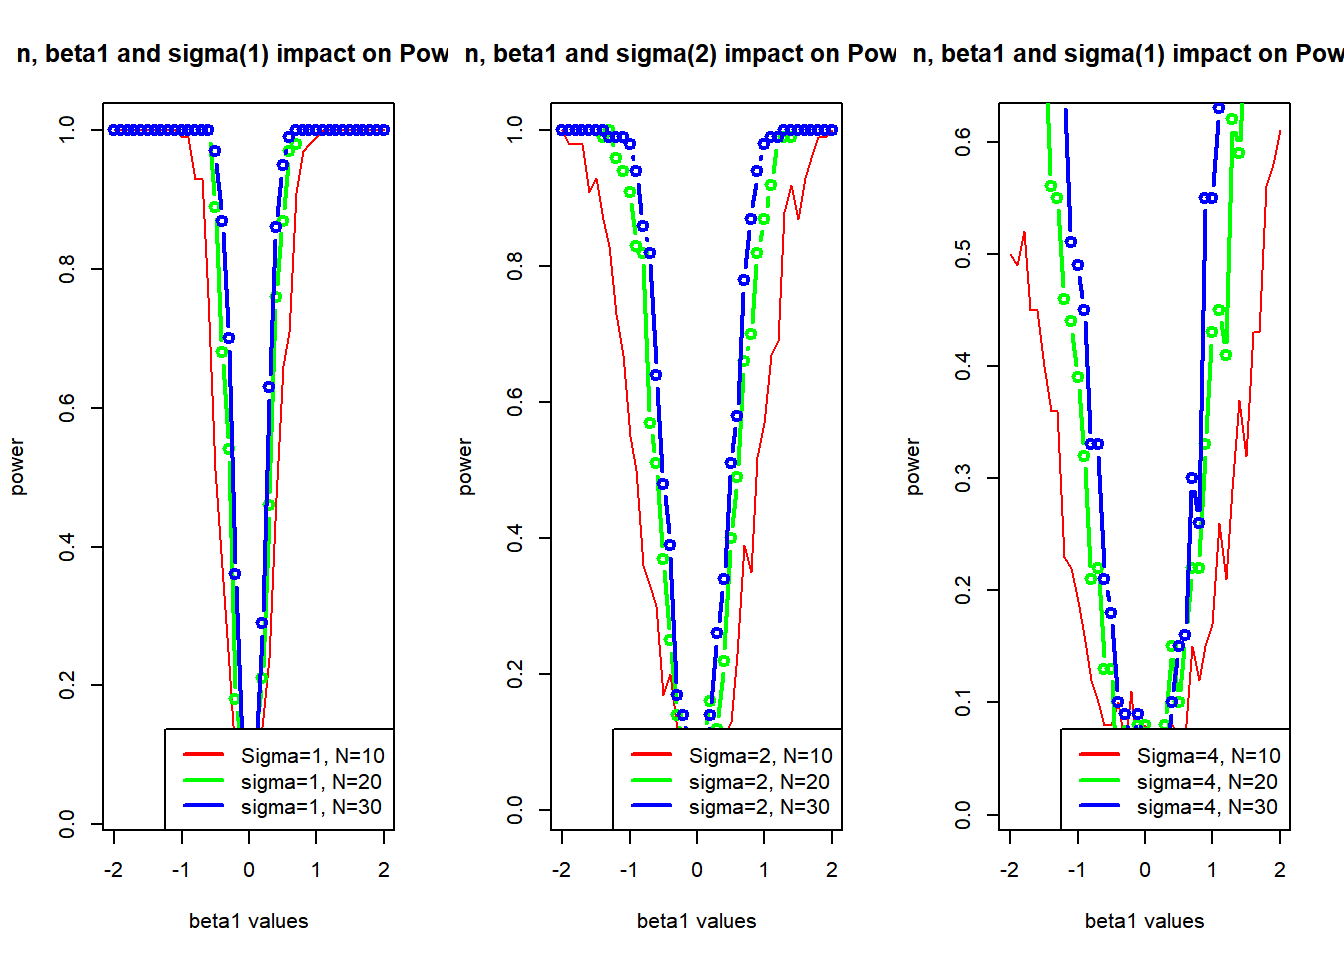
\includegraphics{w03-hw-bollamr2_files/figure-latex/unnamed-chunk-10-1.pdf}

\textbf{(g)} Use a \(t\) test to test:

\begin{itemize}
\tightlist
\item
  \(H_0: \beta_1 = 4\)
\item
  \(H_1: \beta_1 \neq 4\)
\end{itemize}

Report the following:

\begin{itemize}
\tightlist
\item
  The value of the test statistic
\item
  The p-value of the test
\item
  A statistical decision at \(\alpha = 0.05\)
\end{itemize}

When reporting these, you should explicitly state them in your document,
not assume that a reader will find and interpret them from a large block
of \texttt{R} output.

\begin{Shaded}
\begin{Highlighting}[]
\NormalTok{beta_}\DecValTok{1}\NormalTok{ =}\StringTok{ }\KeywordTok{coefficients}\NormalTok{(cat_model)[}\DecValTok{2}\NormalTok{]}
\NormalTok{stand_error =}\StringTok{ }\KeywordTok{summary}\NormalTok{(cat_model)}\OperatorTok{$}\NormalTok{coefficients[}\StringTok{"Bwt"}\NormalTok{, }\StringTok{"Std. Error"}\NormalTok{]}
\NormalTok{beta_}\DecValTok{1}\NormalTok{_hat_t =}\StringTok{ }\NormalTok{(beta_}\DecValTok{1} \OperatorTok{-}\StringTok{ }\DecValTok{4}\NormalTok{) }\OperatorTok{/}\StringTok{ }\NormalTok{stand_error}
\NormalTok{beta_}\DecValTok{1}\NormalTok{_hat_t}
\end{Highlighting}
\end{Shaded}

\begin{verbatim}
##       Bwt 
## 0.1361084
\end{verbatim}

\begin{Shaded}
\begin{Highlighting}[]
\NormalTok{p_value =}\StringTok{ }\DecValTok{2} \OperatorTok{*}\StringTok{ }\KeywordTok{pt}\NormalTok{(}\KeywordTok{abs}\NormalTok{(beta_}\DecValTok{1}\NormalTok{_hat_t), }\DataTypeTok{df =} \KeywordTok{length}\NormalTok{(}\KeywordTok{resid}\NormalTok{(cat_model)) }\OperatorTok{-}\StringTok{ }\DecValTok{2}\NormalTok{, }\DataTypeTok{lower.tail =} \OtherTok{FALSE}\NormalTok{)}
\NormalTok{p_value}
\end{Highlighting}
\end{Shaded}

\begin{verbatim}
##       Bwt 
## 0.8919283
\end{verbatim}

The value of the test statistic is 0.1361084

The p-value of the test is 0.8919283.

At statistical decision at \(\alpha = 0.05\) is ``Fail to reject H0''

\begin{center}\rule{0.5\linewidth}{0.5pt}\end{center}

\hypertarget{exercise-2-more-lm-for-inference}{%
\subsection{\texorpdfstring{Exercise 2 (More \texttt{lm} for
Inference)}{Exercise 2 (More lm for Inference)}}\label{exercise-2-more-lm-for-inference}}

For this exercise we will use the \texttt{Ozone} dataset from the
\texttt{mlbench} package. You should use \texttt{?Ozone} to learn about
the background of this dataset. You may need to install the
\texttt{mlbench} package. If you do so, do not include code to install
the package in your \texttt{R} Markdown document.

For simplicity, we will re-perform the data cleaning done in the
previous homework.

\begin{Shaded}
\begin{Highlighting}[]
\KeywordTok{data}\NormalTok{(Ozone, }\DataTypeTok{package =} \StringTok{"mlbench"}\NormalTok{)}
\NormalTok{Ozone =}\StringTok{ }\NormalTok{Ozone[, }\KeywordTok{c}\NormalTok{(}\DecValTok{4}\NormalTok{, }\DecValTok{6}\NormalTok{, }\DecValTok{7}\NormalTok{, }\DecValTok{8}\NormalTok{)]}
\KeywordTok{colnames}\NormalTok{(Ozone) =}\StringTok{ }\KeywordTok{c}\NormalTok{(}\StringTok{"ozone"}\NormalTok{, }\StringTok{"wind"}\NormalTok{, }\StringTok{"humidity"}\NormalTok{, }\StringTok{"temp"}\NormalTok{)}
\NormalTok{Ozone =}\StringTok{ }\NormalTok{Ozone[}\KeywordTok{complete.cases}\NormalTok{(Ozone), ]}
\end{Highlighting}
\end{Shaded}

\textbf{(a)} Fit the following simple linear regression model in
\texttt{R}. Use the ozone measurement as the response and wind speed as
the predictor.

\[
Y_i = \beta_0 + \beta_1 x_i + \epsilon_i
\]

Store the results in a variable called \texttt{ozone\_wind\_model}. Use
a \(t\) test to test the significance of the regression. Report the
following:

\begin{itemize}
\tightlist
\item
  The null and alternative hypotheses
\item
  The value of the test statistic
\item
  The p-value of the test
\item
  A statistical decision at \(\alpha = 0.01\)
\item
  A conclusion in the context of the problem
\end{itemize}

When reporting these, you should explicitly state them in your document,
not assume that a reader will find and interpret them from a large block
of \texttt{R} output.

\begin{Shaded}
\begin{Highlighting}[]
\NormalTok{ozone_model =}\StringTok{ }\KeywordTok{lm}\NormalTok{(ozone }\OperatorTok{~}\StringTok{ }\NormalTok{wind, }\DataTypeTok{data =}\NormalTok{ Ozone)}
\KeywordTok{summary}\NormalTok{(ozone_model)}\OperatorTok{$}\NormalTok{coefficients[}\StringTok{"wind"}\NormalTok{, }\StringTok{"t value"}\NormalTok{]}
\end{Highlighting}
\end{Shaded}

\begin{verbatim}
## [1] -0.2189811
\end{verbatim}

\begin{Shaded}
\begin{Highlighting}[]
\KeywordTok{summary}\NormalTok{(ozone_model)}\OperatorTok{$}\NormalTok{coefficients[}\StringTok{"wind"}\NormalTok{, }\StringTok{"Pr(>|t|)"}\NormalTok{]}
\end{Highlighting}
\end{Shaded}

\begin{verbatim}
## [1] 0.8267954
\end{verbatim}

H0: \(\hat{\beta}_1\) = 0, \[Y_i = \beta_0 + \epsilon_i\]

H1: \(\hat{\beta}_1\) != 0, \[Y_i = \beta_0 + \beta_1 x_i + \epsilon_i\]

The value of the test statistic is -0.2189811

The p-value of the test is 0.8267954

Statistical Decision at alpha = 0.01 is Fail to Reject H0

Conclusion in the context of the problem: there exists a NO linear
relationship between ozone and wind speed

\textbf{(b)} Fit the following simple linear regression model in
\texttt{R}. Use the ozone measurement as the response and temperature as
the predictor.

\[
Y_i = \beta_0 + \beta_1 x_i + \epsilon_i
\]

Store the results in a variable called \texttt{ozone\_temp\_model}. Use
a \(t\) test to test the significance of the regression. Report the
following:

\begin{itemize}
\tightlist
\item
  The null and alternative hypotheses
\item
  The value of the test statistic
\item
  The p-value of the test
\item
  A statistical decision at \(\alpha = 0.01\)
\item
  A conclusion in the context of the problem
\end{itemize}

When reporting these, you should explicitly state them in your document,
not assume that a reader will find and interpret them from a large block
of \texttt{R} output.

\begin{Shaded}
\begin{Highlighting}[]
\NormalTok{ozone_model =}\StringTok{ }\KeywordTok{lm}\NormalTok{(ozone }\OperatorTok{~}\StringTok{ }\NormalTok{temp, }\DataTypeTok{data =}\NormalTok{ Ozone)}
\KeywordTok{summary}\NormalTok{(ozone_model)}\OperatorTok{$}\NormalTok{coefficients[}\StringTok{"temp"}\NormalTok{, }\StringTok{"t value"}\NormalTok{]}
\end{Highlighting}
\end{Shaded}

\begin{verbatim}
## [1] 22.84896
\end{verbatim}

\begin{Shaded}
\begin{Highlighting}[]
\KeywordTok{summary}\NormalTok{(ozone_model)}\OperatorTok{$}\NormalTok{coefficients[}\StringTok{"temp"}\NormalTok{, }\StringTok{"Pr(>|t|)"}\NormalTok{]}
\end{Highlighting}
\end{Shaded}

\begin{verbatim}
## [1] 8.153764e-71
\end{verbatim}

H0: \(\hat{\beta}_1\) = 0, \[Y_i = \beta_0 + \epsilon_i\]

H1: \(\hat{\beta}_1\) != 0, \[Y_i = \beta_0 + \beta_1 x_i + \epsilon_i\]

The value of the test statistic is 22.84896

The p-value of the test is 8.153764e-71

Statistical Decision at alpha = 0.01 is Reject H0

Conclusion in the context of the problem: there exists a linear
relationship between ozone and temperature

\begin{center}\rule{0.5\linewidth}{0.5pt}\end{center}

\hypertarget{exercise-3-simulating-sampling-distributions}{%
\subsection{Exercise 3 (Simulating Sampling
Distributions)}\label{exercise-3-simulating-sampling-distributions}}

For this exercise we will simulate data from the following model:

\[
Y_i = \beta_0 + \beta_1 x_i + \epsilon_i
\]

Where \(\epsilon_i \sim N(0, \sigma^2).\) Also, the parameters are known
to be:

\begin{itemize}
\tightlist
\item
  \(\beta_0 = -5\)
\item
  \(\beta_1 = 3.25\)
\item
  \(\sigma^2 = 16\)
\end{itemize}

We will use samples of size \(n = 50\).

\textbf{(a)} Simulate this model \(2000\) times. Each time use
\texttt{lm()} to fit a simple linear regression model, then store the
value of \(\hat{\beta}_0\) and \(\hat{\beta}_1\). Set a seed using
\textbf{your} birthday before performing the simulation. Note, we are
simulating the \(x\) values once, and then they remain fixed for the
remainder of the exercise.

\begin{Shaded}
\begin{Highlighting}[]
\NormalTok{birthday =}\StringTok{ }\DecValTok{19830611} \CommentTok{#18760613}
\KeywordTok{set.seed}\NormalTok{(birthday)}
\NormalTok{n =}\StringTok{ }\DecValTok{50}
\NormalTok{x =}\StringTok{ }\KeywordTok{seq}\NormalTok{(}\DecValTok{0}\NormalTok{, }\DecValTok{10}\NormalTok{, }\DataTypeTok{length =}\NormalTok{ n)}

\NormalTok{beta_}\DecValTok{0}\NormalTok{ =}\StringTok{ }\DecValTok{-5}
\NormalTok{beta_}\DecValTok{1}\NormalTok{ =}\StringTok{ }\FloatTok{3.25}
\NormalTok{sigma =}\StringTok{ }\DecValTok{4}

\NormalTok{num_samples =}\StringTok{ }\DecValTok{2000}
\NormalTok{beta_}\DecValTok{0}\NormalTok{_hats =}\StringTok{ }\KeywordTok{rep}\NormalTok{(}\DecValTok{0}\NormalTok{, num_samples)}
\NormalTok{beta_}\DecValTok{1}\NormalTok{_hats =}\StringTok{ }\KeywordTok{rep}\NormalTok{(}\DecValTok{0}\NormalTok{, num_samples)}

\ControlFlowTok{for}\NormalTok{(i }\ControlFlowTok{in} \DecValTok{1}\OperatorTok{:}\NormalTok{num_samples) \{}
\NormalTok{  eps =}\StringTok{ }\KeywordTok{rnorm}\NormalTok{(n, }\DataTypeTok{mean =} \DecValTok{0}\NormalTok{, }\DataTypeTok{sd =}\NormalTok{ sigma)}
\NormalTok{  y =}\StringTok{ }\NormalTok{beta_}\DecValTok{0} \OperatorTok{+}\StringTok{ }\NormalTok{beta_}\DecValTok{1} \OperatorTok{*}\StringTok{ }\NormalTok{x }\OperatorTok{+}\StringTok{ }\NormalTok{eps}
\NormalTok{  sim_model =}\StringTok{ }\KeywordTok{lm}\NormalTok{(y }\OperatorTok{~}\StringTok{ }\NormalTok{x)}
\NormalTok{  beta_}\DecValTok{0}\NormalTok{_hats[i] =}\StringTok{ }\KeywordTok{coef}\NormalTok{(sim_model)[}\DecValTok{1}\NormalTok{]}
\NormalTok{  beta_}\DecValTok{1}\NormalTok{_hats[i] =}\StringTok{ }\KeywordTok{coef}\NormalTok{(sim_model)[}\DecValTok{2}\NormalTok{]}
\NormalTok{\}}
\end{Highlighting}
\end{Shaded}

\textbf{(b)} Create a table that summarizes the results of the
simulations. The table should have two columns, one for
\(\hat{\beta}_0\) and one for \(\hat{\beta}_1\). The table should have
four rows:

\begin{itemize}
\tightlist
\item
  A row for the true expected value given the known values of \(x\)
\item
  A row for the mean of the simulated values
\item
  A row for the true standard deviation given the known values of \(x\)
\item
  A row for the standard deviation of the simulated values
\end{itemize}

\begin{Shaded}
\begin{Highlighting}[]
\NormalTok{Sxx =}\StringTok{ }\KeywordTok{sum}\NormalTok{((x }\OperatorTok{-}\StringTok{ }\KeywordTok{mean}\NormalTok{(x)) }\OperatorTok{^}\StringTok{ }\DecValTok{2}\NormalTok{)}
\NormalTok{var_beta_}\DecValTok{1}\NormalTok{_hat =}\StringTok{ }\NormalTok{(sigma }\OperatorTok{^}\StringTok{ }\DecValTok{2}\NormalTok{)}\OperatorTok{/}\NormalTok{Sxx}
\NormalTok{var_beta_}\DecValTok{0}\NormalTok{_hat =}\StringTok{ }\NormalTok{(sigma }\OperatorTok{^}\StringTok{ }\DecValTok{2}\NormalTok{)}\OperatorTok{*}\NormalTok{((}\DecValTok{1}\OperatorTok{/}\NormalTok{n) }\OperatorTok{+}\StringTok{ }\NormalTok{(}\KeywordTok{mean}\NormalTok{(x)}\OperatorTok{^}\DecValTok{2}\OperatorTok{/}\NormalTok{Sxx))}
\NormalTok{data_summary =}\StringTok{ }\KeywordTok{data.frame}\NormalTok{(}\DataTypeTok{value =} \KeywordTok{c}\NormalTok{(}\StringTok{"E of known values"}\NormalTok{, }\StringTok{"mean of simulated vlaues"}\NormalTok{, }\StringTok{"SD of known vlaues"}\NormalTok{, }\StringTok{"sd of simulated values"}\NormalTok{),}
                          \DataTypeTok{beta_0_hat =} \KeywordTok{c}\NormalTok{(beta_}\DecValTok{0}\NormalTok{, }\KeywordTok{mean}\NormalTok{(beta_}\DecValTok{0}\NormalTok{_hats), var_beta_}\DecValTok{0}\NormalTok{_hat, }\KeywordTok{sd}\NormalTok{(beta_}\DecValTok{0}\NormalTok{_hats)),}
                          \DataTypeTok{beta_1_hat =} \KeywordTok{c}\NormalTok{(beta_}\DecValTok{1}\NormalTok{, }\KeywordTok{mean}\NormalTok{(beta_}\DecValTok{1}\NormalTok{_hats), var_beta_}\DecValTok{1}\NormalTok{_hat, }\KeywordTok{sd}\NormalTok{(beta_}\DecValTok{1}\NormalTok{_hats))}
\NormalTok{                          )}
\KeywordTok{library}\NormalTok{(knitr)}
\KeywordTok{kable}\NormalTok{(data_summary)}
\end{Highlighting}
\end{Shaded}

\begin{longtable}[]{@{}lrr@{}}
\toprule
value & beta\_0\_hat & beta\_1\_hat\tabularnewline
\midrule
\endhead
E of known values & -5.000000 & 3.2500000\tabularnewline
mean of simulated vlaues & -5.018445 & 3.2533514\tabularnewline
SD of known vlaues & 1.242353 & 0.0368941\tabularnewline
sd of simulated values & 1.097462 & 0.1919585\tabularnewline
\bottomrule
\end{longtable}

\textbf{(c)} Plot two histograms side-by-side:

\begin{itemize}
\tightlist
\item
  A histogram of your simulated values for \(\hat{\beta}_0\). Add the
  normal curve for the true sampling distribution of \(\hat{\beta}_0\).
\item
  A histogram of your simulated values for \(\hat{\beta}_1\). Add the
  normal curve for the true sampling distribution of \(\hat{\beta}_1\).
\end{itemize}

\begin{Shaded}
\begin{Highlighting}[]
\KeywordTok{hist}\NormalTok{(beta_}\DecValTok{0}\NormalTok{_hats, }\DataTypeTok{prob =} \OtherTok{TRUE}\NormalTok{, }\DataTypeTok{breaks =} \DecValTok{25}\NormalTok{, }\DataTypeTok{col =} \StringTok{"grey"}\NormalTok{, }\DataTypeTok{border =} \StringTok{"brown"}\NormalTok{, }\DataTypeTok{xlab =} \KeywordTok{expression}\NormalTok{(}\KeywordTok{hat}\NormalTok{(beta)[}\DecValTok{0}\NormalTok{]), }\DataTypeTok{main =} \StringTok{""}\NormalTok{)}
\KeywordTok{curve}\NormalTok{(}\KeywordTok{dnorm}\NormalTok{(x, }\DataTypeTok{mean =}\NormalTok{ beta_}\DecValTok{0}\NormalTok{, }\DataTypeTok{sd =} \KeywordTok{sqrt}\NormalTok{(var_beta_}\DecValTok{0}\NormalTok{_hat)), }\DataTypeTok{col =} \StringTok{"darkorange"}\NormalTok{, }\DataTypeTok{add =} \OtherTok{TRUE}\NormalTok{, }\DataTypeTok{lwd =} \DecValTok{3}\NormalTok{)}
\end{Highlighting}
\end{Shaded}

\includegraphics{w03-hw-bollamr2_files/figure-latex/unnamed-chunk-17-1.pdf}

\begin{Shaded}
\begin{Highlighting}[]
\KeywordTok{hist}\NormalTok{(beta_}\DecValTok{1}\NormalTok{_hats, }\DataTypeTok{prob =} \OtherTok{TRUE}\NormalTok{, }\DataTypeTok{breaks =} \DecValTok{25}\NormalTok{, }\DataTypeTok{col =} \StringTok{"grey"}\NormalTok{, }\DataTypeTok{border =} \StringTok{"brown"}\NormalTok{, }\DataTypeTok{xlab =} \KeywordTok{expression}\NormalTok{(}\KeywordTok{hat}\NormalTok{(beta)[}\DecValTok{1}\NormalTok{]), }\DataTypeTok{main =} \StringTok{""}\NormalTok{)}
\KeywordTok{curve}\NormalTok{(}\KeywordTok{dnorm}\NormalTok{(x, }\DataTypeTok{mean =}\NormalTok{ beta_}\DecValTok{1}\NormalTok{, }\DataTypeTok{sd =} \KeywordTok{sqrt}\NormalTok{(var_beta_}\DecValTok{1}\NormalTok{_hat)), }\DataTypeTok{col =} \StringTok{"darkorange"}\NormalTok{, }\DataTypeTok{add =} \OtherTok{TRUE}\NormalTok{, }\DataTypeTok{lwd =} \DecValTok{3}\NormalTok{)}
\end{Highlighting}
\end{Shaded}

\includegraphics{w03-hw-bollamr2_files/figure-latex/unnamed-chunk-17-2.pdf}

\begin{center}\rule{0.5\linewidth}{0.5pt}\end{center}

\hypertarget{exercise-4-simulating-confidence-intervals}{%
\subsection{Exercise 4 (Simulating Confidence
Intervals)}\label{exercise-4-simulating-confidence-intervals}}

For this exercise we will simulate data from the following model:

\[
Y_i = \beta_0 + \beta_1 x_i + \epsilon_i
\]

Where \(\epsilon_i \sim N(0, \sigma^2).\) Also, the parameters are known
to be:

\begin{itemize}
\tightlist
\item
  \(\beta_0 = 5\)
\item
  \(\beta_1 = 2\)
\item
  \(\sigma^2 = 9\)
\end{itemize}

We will use samples of size \(n = 25\).

Our goal here is to use simulation to verify that the confidence
intervals really do have their stated confidence level. Do \textbf{not}
use the \texttt{confint()} function for this entire exercise.

\textbf{(a)} Simulate this model \(2500\) times. Each time use
\texttt{lm()} to fit a simple linear regression model, then store the
value of \(\hat{\beta}_1\) and \(s_e\). Set a seed using \textbf{your}
birthday before performing the simulation. Note, we are simulating the
\(x\) values once, and then they remain fixed for the remainder of the
exercise.

\begin{Shaded}
\begin{Highlighting}[]
\NormalTok{birthday =}\StringTok{ }\DecValTok{19830611} \CommentTok{#18760613}
\KeywordTok{set.seed}\NormalTok{(birthday)}
\NormalTok{n =}\StringTok{ }\DecValTok{25}
\NormalTok{x =}\StringTok{ }\KeywordTok{seq}\NormalTok{(}\DecValTok{0}\NormalTok{, }\FloatTok{2.5}\NormalTok{, }\DataTypeTok{length =}\NormalTok{ n)}

\NormalTok{Sxx =}\StringTok{ }\KeywordTok{sum}\NormalTok{((x }\OperatorTok{-}\StringTok{ }\KeywordTok{mean}\NormalTok{(x)) }\OperatorTok{^}\StringTok{ }\DecValTok{2}\NormalTok{)}
\NormalTok{beta_}\DecValTok{0}\NormalTok{ =}\StringTok{ }\DecValTok{5}
\NormalTok{beta_}\DecValTok{1}\NormalTok{ =}\StringTok{ }\DecValTok{2}
\NormalTok{sigma =}\StringTok{ }\DecValTok{3} 

\NormalTok{num_samples =}\StringTok{ }\DecValTok{2500}
\NormalTok{beta_hat_}\DecValTok{1}\NormalTok{ =}\StringTok{ }\KeywordTok{rep}\NormalTok{(}\DecValTok{0}\NormalTok{, num_samples)}
\NormalTok{s_e =}\StringTok{ }\KeywordTok{rep}\NormalTok{(}\DecValTok{0}\NormalTok{, num_samples)}
\ControlFlowTok{for}\NormalTok{ (i }\ControlFlowTok{in} \DecValTok{1}\OperatorTok{:}\NormalTok{num_samples) \{}
\NormalTok{  y =}\StringTok{ }\NormalTok{beta_}\DecValTok{0} \OperatorTok{+}\StringTok{ }\NormalTok{beta_}\DecValTok{1} \OperatorTok{*}\StringTok{ }\NormalTok{x }\OperatorTok{+}\StringTok{ }\KeywordTok{rnorm}\NormalTok{(n, }\DecValTok{0}\NormalTok{, sigma)}
\NormalTok{  sim_model =}\StringTok{ }\KeywordTok{lm}\NormalTok{(y }\OperatorTok{~}\StringTok{ }\NormalTok{x)}
\NormalTok{  beta_}\DecValTok{1}\NormalTok{_hats[i] =}\StringTok{ }\KeywordTok{coef}\NormalTok{(sim_model)[}\DecValTok{2}\NormalTok{]}
\NormalTok{  s_e[i] =}\StringTok{ }\KeywordTok{summary}\NormalTok{(sim_model)}\OperatorTok{$}\NormalTok{sigma}
\NormalTok{\}}
\end{Highlighting}
\end{Shaded}

\textbf{(b)} For each of the \(\hat{\beta}_1\) that you simulated,
calculate a 95\% confidence interval. Store the lower limits in a vector
\texttt{lower\_95} and the upper limits in a vector \texttt{upper\_95}.
Some hints:

\begin{itemize}
\tightlist
\item
  You will need to use \texttt{qt()} to calculate the critical value,
  which will be the same for each interval.
\item
  Remember that \texttt{x} is fixed, so \(S_{xx}\) will be the same for
  each interval.
\item
  You could, but do not need to write a \texttt{for} loop. Remember
  vectorized operations.
\end{itemize}

\begin{Shaded}
\begin{Highlighting}[]
\CommentTok{#confint(sim_model, parm = "(Intercept)", level = 0.95)}
\NormalTok{alpha =}\StringTok{ }\FloatTok{0.05}
\NormalTok{crit =}\StringTok{ }\OperatorTok{-}\KeywordTok{qt}\NormalTok{(alpha }\OperatorTok{/}\StringTok{ }\DecValTok{2}\NormalTok{, }\DataTypeTok{df =}\NormalTok{ n }\OperatorTok{-}\StringTok{ }\DecValTok{2}\NormalTok{)}
\NormalTok{lower_}\DecValTok{95}\NormalTok{ =}\StringTok{ }\NormalTok{beta_}\DecValTok{1}\NormalTok{_hats }\OperatorTok{-}\StringTok{ }\NormalTok{crit }\OperatorTok{*}\StringTok{ }\NormalTok{s_e }\OperatorTok{/}\StringTok{ }\KeywordTok{sqrt}\NormalTok{(Sxx)}
\NormalTok{upper_}\DecValTok{95}\NormalTok{ =}\StringTok{ }\NormalTok{beta_}\DecValTok{1}\NormalTok{_hats }\OperatorTok{+}\StringTok{ }\NormalTok{crit }\OperatorTok{*}\StringTok{ }\NormalTok{s_e }\OperatorTok{/}\StringTok{ }\KeywordTok{sqrt}\NormalTok{(Sxx)}
\end{Highlighting}
\end{Shaded}

\textbf{(c)} What proportion of these intervals contains the true value
of \(\beta_1\)?

\begin{Shaded}
\begin{Highlighting}[]
\KeywordTok{mean}\NormalTok{(lower_}\DecValTok{95} \OperatorTok{<}\StringTok{ }\NormalTok{beta_}\DecValTok{1} \OperatorTok{&}\StringTok{ }\NormalTok{beta_}\DecValTok{1} \OperatorTok{<}\StringTok{ }\NormalTok{upper_}\DecValTok{95}\NormalTok{)}
\end{Highlighting}
\end{Shaded}

\begin{verbatim}
## [1] 0.9496
\end{verbatim}

The result is 94.96\% very close to 95\%

\textbf{(d)} Based on these intervals, what proportion of the
simulations would reject the test \(H_0: \beta_1 = 0\) vs
\(H_1: \beta_1 \neq 0\) at \(\alpha = 0.05\)?

\begin{Shaded}
\begin{Highlighting}[]
\DecValTok{1} \OperatorTok{-}\StringTok{ }\KeywordTok{mean}\NormalTok{(lower_}\DecValTok{95} \OperatorTok{<}\StringTok{ }\DecValTok{0} \OperatorTok{&}\StringTok{ }\DecValTok{0} \OperatorTok{<}\StringTok{ }\NormalTok{upper_}\DecValTok{95}\NormalTok{)}
\end{Highlighting}
\end{Shaded}

\begin{verbatim}
## [1] 0.6672
\end{verbatim}

\textbf{(e)} For each of the \(\hat{\beta}_1\) that you simulated,
calculate a 99\% confidence interval. Store the lower limits in a vector
\texttt{lower\_99} and the upper limits in a vector \texttt{upper\_99}.

\begin{Shaded}
\begin{Highlighting}[]
\NormalTok{alpha =}\StringTok{ }\FloatTok{0.01}
\NormalTok{crit =}\StringTok{ }\OperatorTok{-}\KeywordTok{qt}\NormalTok{(alpha }\OperatorTok{/}\StringTok{ }\DecValTok{2}\NormalTok{, }\DataTypeTok{df =}\NormalTok{ n }\OperatorTok{-}\StringTok{ }\DecValTok{2}\NormalTok{)}
\NormalTok{lower_}\DecValTok{99}\NormalTok{ =}\StringTok{ }\NormalTok{beta_}\DecValTok{1}\NormalTok{_hats }\OperatorTok{-}\StringTok{ }\NormalTok{crit }\OperatorTok{*}\StringTok{ }\NormalTok{s_e }\OperatorTok{/}\StringTok{ }\KeywordTok{sqrt}\NormalTok{(Sxx)}
\NormalTok{upper_}\DecValTok{99}\NormalTok{ =}\StringTok{ }\NormalTok{beta_}\DecValTok{1}\NormalTok{_hats }\OperatorTok{+}\StringTok{ }\NormalTok{crit }\OperatorTok{*}\StringTok{ }\NormalTok{s_e }\OperatorTok{/}\StringTok{ }\KeywordTok{sqrt}\NormalTok{(Sxx)}
\end{Highlighting}
\end{Shaded}

\textbf{(f)} What proportion of these intervals contains the true value
of \(\beta_1\)?

\begin{Shaded}
\begin{Highlighting}[]
\KeywordTok{mean}\NormalTok{(lower_}\DecValTok{99} \OperatorTok{<}\StringTok{ }\NormalTok{beta_}\DecValTok{1} \OperatorTok{&}\StringTok{ }\NormalTok{beta_}\DecValTok{1} \OperatorTok{<}\StringTok{ }\NormalTok{upper_}\DecValTok{99}\NormalTok{)}
\end{Highlighting}
\end{Shaded}

\begin{verbatim}
## [1] 0.9868
\end{verbatim}

The result is 98.68\%, very close to 99\%.

\textbf{(g)} Based on these intervals, what proportion of the
simulations would reject the test \(H_0: \beta_1 = 0\) vs
\(H_1: \beta_1 \neq 0\) at \(\alpha = 0.01\)?

\begin{Shaded}
\begin{Highlighting}[]
\DecValTok{1} \OperatorTok{-}\StringTok{ }\KeywordTok{mean}\NormalTok{(lower_}\DecValTok{99} \OperatorTok{<}\StringTok{ }\DecValTok{0} \OperatorTok{&}\StringTok{ }\DecValTok{0} \OperatorTok{<}\StringTok{ }\NormalTok{upper_}\DecValTok{99}\NormalTok{)}
\end{Highlighting}
\end{Shaded}

\begin{verbatim}
## [1] 0.3996
\end{verbatim}

\begin{center}\rule{0.5\linewidth}{0.5pt}\end{center}

\hypertarget{exercise-5-prediction-intervals-without-predict}{%
\subsection{\texorpdfstring{Exercise 5 (Prediction Intervals ``without''
\texttt{predict})}{Exercise 5 (Prediction Intervals ``without'' predict)}}\label{exercise-5-prediction-intervals-without-predict}}

Write a function named \texttt{calc\_pred\_int} that performs calculates
prediction intervals:

\[
\hat{y}(x) \pm t_{\alpha/2, n - 2} \cdot s_e\sqrt{1 + \frac{1}{n}+\frac{(x-\bar{x})^2}{S_{xx}}}.
\]

for the linear model

\[
Y_i = \beta_0 + \beta_1 x_i + \epsilon_i.
\]

\textbf{(a)} Write this function. You may use the \texttt{predict()}
function, but you may \textbf{not} supply a value for the \texttt{level}
argument of \texttt{predict()}. (You can certainly use
\texttt{predict()} any way you would like in order to check your work.)

The function should take three inputs:

\begin{itemize}
\tightlist
\item
  \texttt{model}, a model object that is the result of fitting the SLR
  model with \texttt{lm()}
\item
  \texttt{newdata}, a data frame with a single observation (row)

  \begin{itemize}
  \tightlist
  \item
    This data frame will need to have a variable (column) with the same
    name as the data used to fit \texttt{model}.
  \end{itemize}
\item
  \texttt{level}, the level (0.90, 0.95, etc) for the interval with a
  default value of \texttt{0.95}
\end{itemize}

The function should return a named vector with three elements:

\begin{itemize}
\tightlist
\item
  \texttt{estimate}, the midpoint of the interval
\item
  \texttt{lower}, the lower bound of the interval
\item
  \texttt{upper}, the upper bound of the interval
\end{itemize}

\begin{Shaded}
\begin{Highlighting}[]
\NormalTok{calc_pred_int =}\StringTok{ }\ControlFlowTok{function}\NormalTok{(model , newdata, }\DataTypeTok{level =} \FloatTok{0.95}\NormalTok{) \{}
  
\NormalTok{  t_}\DecValTok{95}\NormalTok{ =}\StringTok{ }\KeywordTok{abs}\NormalTok{(}\KeywordTok{qt}\NormalTok{(}\FloatTok{0.05}\OperatorTok{/}\DecValTok{2}\NormalTok{, }\DataTypeTok{df =} \KeywordTok{length}\NormalTok{(}\KeywordTok{resid}\NormalTok{(model)) }\OperatorTok{-}\StringTok{ }\DecValTok{2}\NormalTok{))}
\NormalTok{  interval_}\DecValTok{95}\NormalTok{ =}\StringTok{ }\KeywordTok{predict}\NormalTok{(model, newdata, }\DataTypeTok{interval =} \StringTok{"prediction"}\NormalTok{)}
\NormalTok{  lwr_}\DecValTok{95}\NormalTok{ =}\StringTok{ }\NormalTok{interval_}\DecValTok{95}\NormalTok{[}\DecValTok{2}\NormalTok{]}
\NormalTok{  upr_}\DecValTok{95}\NormalTok{ =}\StringTok{ }\NormalTok{interval_}\DecValTok{95}\NormalTok{[}\DecValTok{3}\NormalTok{]}
\NormalTok{  margin =(upr_}\DecValTok{95} \OperatorTok{-}\StringTok{ }\NormalTok{lwr_}\DecValTok{95}\NormalTok{)}\OperatorTok{/}\DecValTok{2}
\NormalTok{  se =}\StringTok{ }\NormalTok{margin}\OperatorTok{/}\NormalTok{t_}\DecValTok{95}

\NormalTok{  alpha =}\StringTok{ }\DecValTok{1} \OperatorTok{-}\StringTok{ }\NormalTok{level}
\NormalTok{  t =}\StringTok{ }\KeywordTok{abs}\NormalTok{(}\KeywordTok{qt}\NormalTok{(alpha}\OperatorTok{/}\DecValTok{2}\NormalTok{, }\DataTypeTok{df =} \KeywordTok{length}\NormalTok{(}\KeywordTok{resid}\NormalTok{(model)) }\OperatorTok{-}\StringTok{ }\DecValTok{2}\NormalTok{))}
  
  \KeywordTok{c}\NormalTok{(}\DataTypeTok{est =}\NormalTok{ interval_}\DecValTok{95}\NormalTok{[}\DecValTok{1}\NormalTok{], }\DataTypeTok{lwr =}\NormalTok{ interval_}\DecValTok{95}\NormalTok{[}\DecValTok{1}\NormalTok{] }\OperatorTok{-}\StringTok{ }\NormalTok{t}\OperatorTok{*}\NormalTok{se , }\DataTypeTok{upr =}\NormalTok{ interval_}\DecValTok{95}\NormalTok{[}\DecValTok{1}\NormalTok{] }\OperatorTok{+}\StringTok{ }\NormalTok{t}\OperatorTok{*}\NormalTok{se)}
\NormalTok{\}}
\end{Highlighting}
\end{Shaded}

\textbf{(b)} After writing the function, run this code:

\begin{Shaded}
\begin{Highlighting}[]
\NormalTok{newcat_}\DecValTok{1}\NormalTok{ =}\StringTok{ }\KeywordTok{data.frame}\NormalTok{(}\DataTypeTok{Bwt =} \FloatTok{4.0}\NormalTok{)}
\KeywordTok{calc_pred_int}\NormalTok{(cat_model, newcat_}\DecValTok{1}\NormalTok{)}
\end{Highlighting}
\end{Shaded}

For some reason result is not output to html page while knitting. Hence
manually copying the result here; No problem in rstudio.

estimate = 15.77959

lower = 12.83018

upper = 18.72900

\textbf{(c)} After writing the function, run this code:

\begin{Shaded}
\begin{Highlighting}[]
\NormalTok{newcat_}\DecValTok{2}\NormalTok{ =}\StringTok{ }\KeywordTok{data.frame}\NormalTok{(}\DataTypeTok{Bwt =} \FloatTok{3.3}\NormalTok{)}
\KeywordTok{calc_pred_int}\NormalTok{(cat_model, newcat_}\DecValTok{2}\NormalTok{, }\DataTypeTok{level =} \FloatTok{0.90}\NormalTok{)}
\end{Highlighting}
\end{Shaded}

For some reason result is not output to html page while knitting. Hence
manually copying the result here; No problem in rstudio.

estimate = 12.95574

lower = 10.53099

upper = 15.38050

\begin{center}\rule{0.5\linewidth}{0.5pt}\end{center}

\end{document}
